\chapter{研究方法示例章}
\label{chap:method}

本章展示研究报告中常用的格式元素，包括图表、公式、算法、代码块等。

\section{图的使用方法}
\subsection{单图插入}
图\ref{fig:single_figure}展示了单图插入的基本格式。
图片应当有清晰的图题，图号按章节编号。

\begin{figure}[htbp]
    \centering
    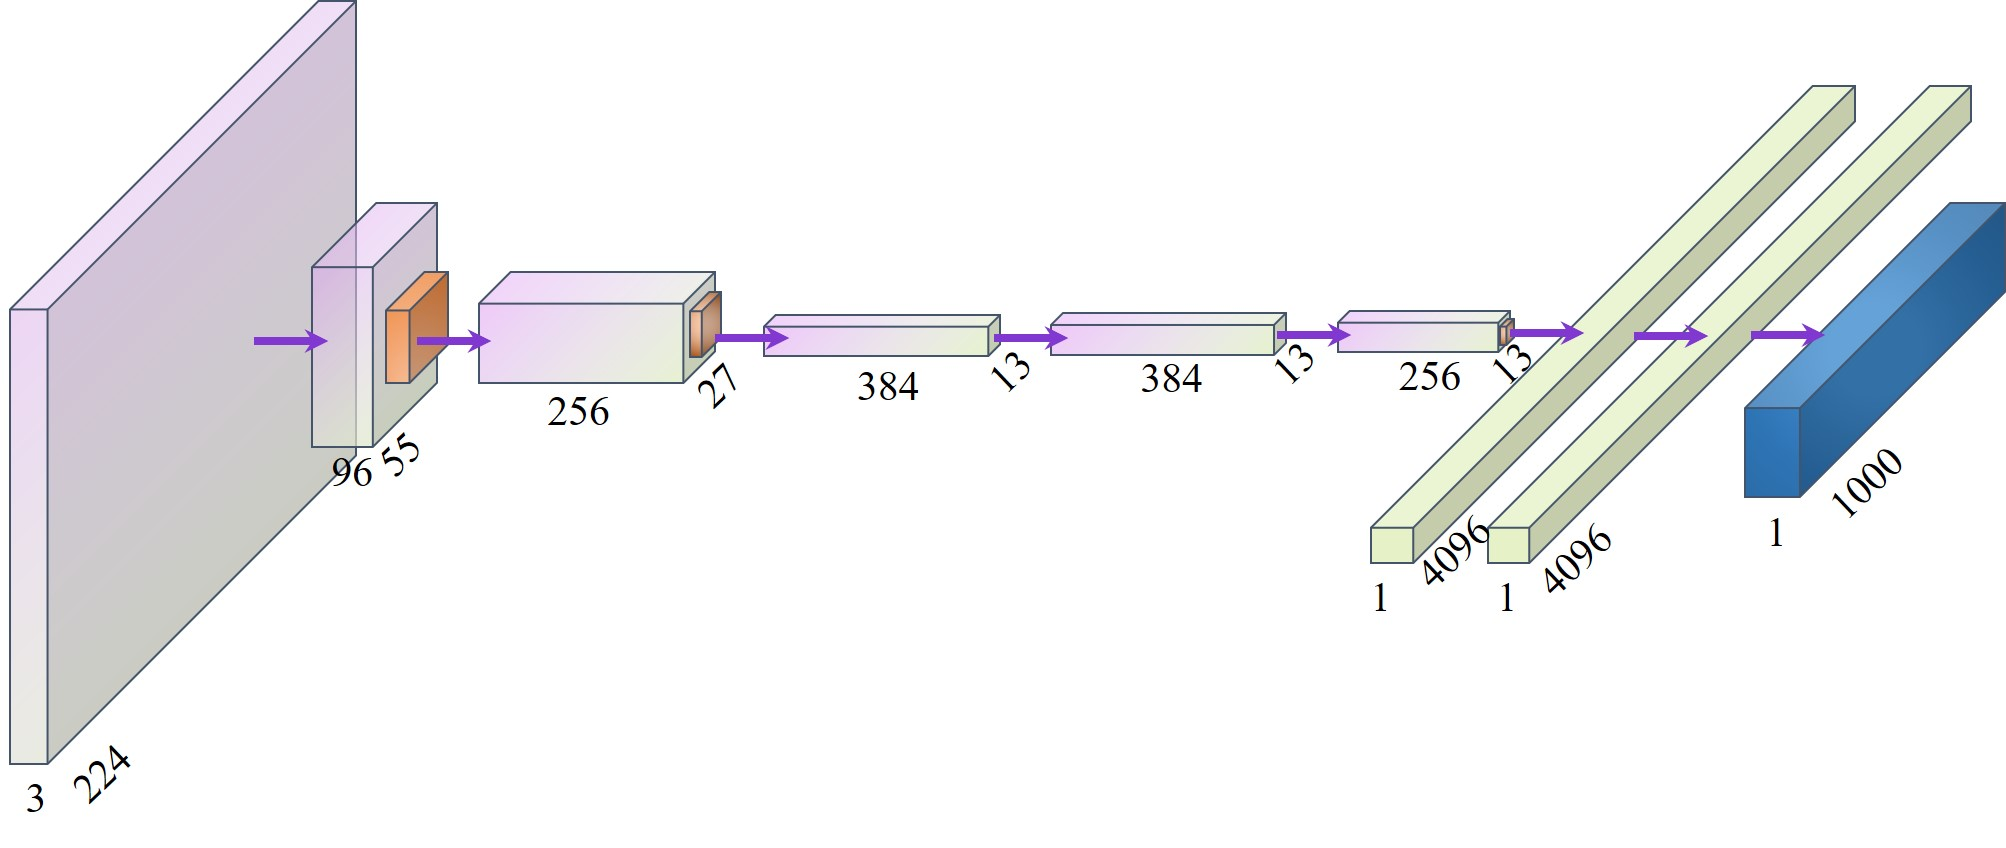
\includegraphics[width=0.5\textwidth]{figures/CNN.jpg}
    \caption{卷积神经网络结构示意图（单图示例）}
    \label{fig:single_figure}
\end{figure}

\subsection{多图并排}
当需要展示多张相关图片时，可采用并排排列的方式。
图\ref{fig:multi_figure}展示了多图并排的格式。

\begin{figure}[htbp]
    \centering
    \begin{subfigure}[b]{0.3\textwidth}
        \centering
        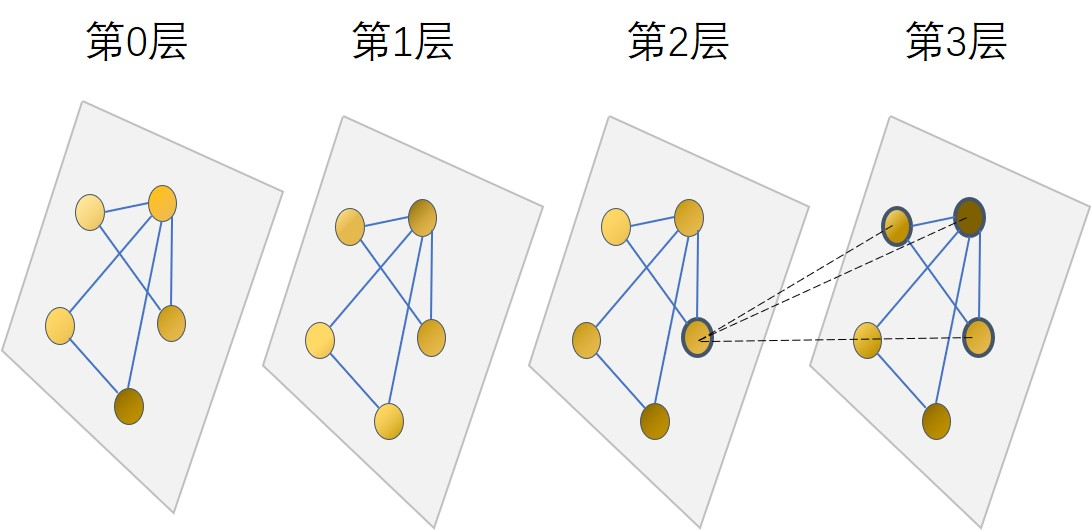
\includegraphics[width=\textwidth]{figures/GNN.jpg}
        \caption{图神经网络}
    \end{subfigure}
    \hfill
    \begin{subfigure}[b]{0.3\textwidth}
        \centering
        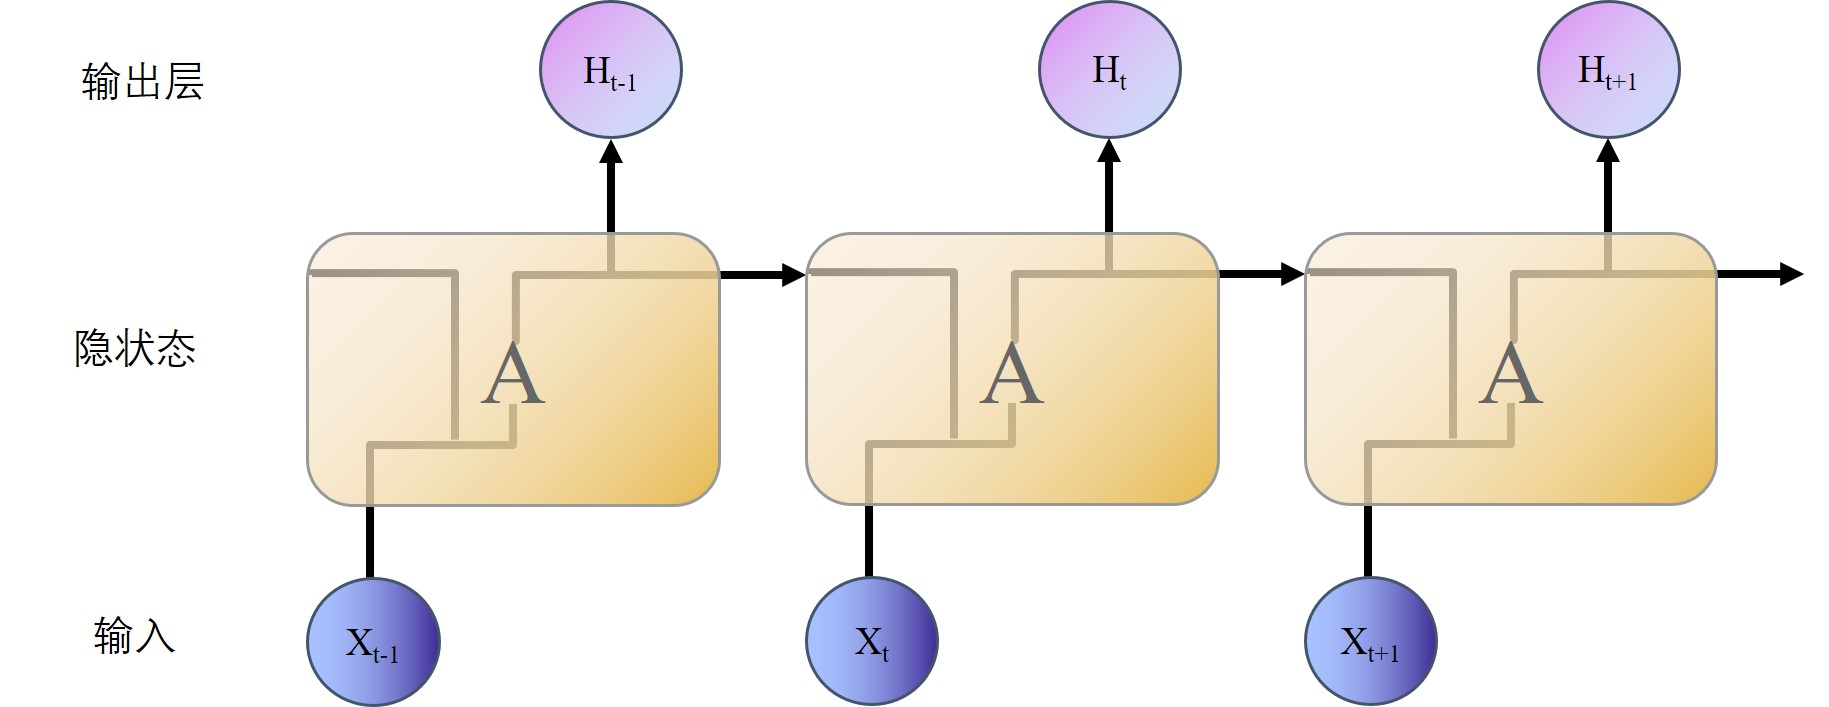
\includegraphics[width=\textwidth]{figures/RNN.jpg}
        \caption{循环神经网络}
    \end{subfigure}
    \hfill
    \begin{subfigure}[b]{0.3\textwidth}
        \centering
        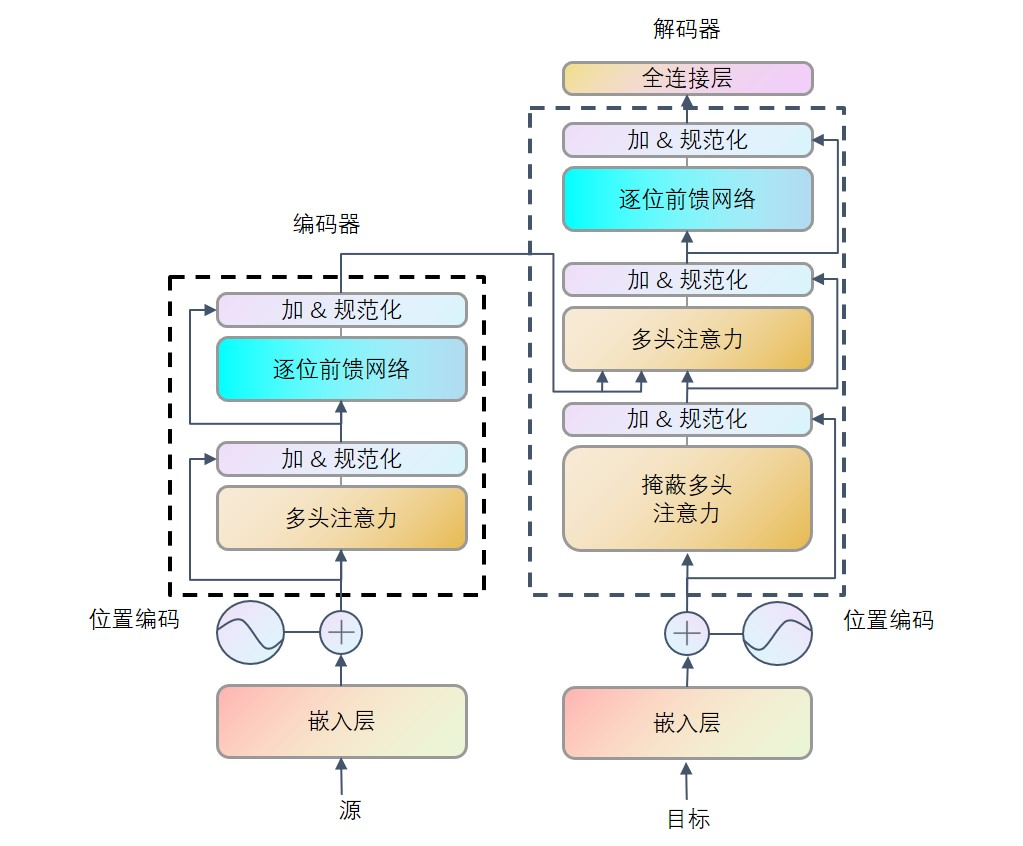
\includegraphics[width=\textwidth]{figures/Transformer.jpg}
        \caption{Transformer}
    \end{subfigure}
    \caption{不同类型神经网络结构示意图（多图并排示例）}
    \label{fig:multi_figure}
\end{figure}

\section{表格的使用方法}
\subsection{基本表格}
表\ref{tab:basic_table}展示了基本表格的格式。
表格应当有清晰的表题，表号按章节编号。

\begin{table}[htbp]
    \caption{基本表格示例}
    \label{tab:basic_table}
    \centering
    \begin{tabular}{lccc}
        \toprule
        参数名称 & 参数值1 & 参数值2 & 参数值3 \\
        \midrule
        参数A & 10 & 20 & 30 \\
        参数B & 40 & 50 & 60 \\
        参数C & 70 & 80 & 90 \\
        \bottomrule
    \end{tabular}
\end{table}

\subsection{三线表}
三线表是学术论文中常用的表格格式，只保留顶线、底线和栏目线。
表\ref{tab:three_line_table}展示了三线表的格式。

\begin{table}[htbp]
    \caption{三线表示例}
    \label{tab:three_line_table}
    \centering
    \begin{tabular}{lcc}
        \toprule
        实验编号 & 测量值1 & 测量值2 \\
        \midrule
        Exp-1 & 100.5 & 98.3 \\
        Exp-2 & 102.1 & 101.7 \\
        Exp-3 & 99.8 & 100.2 \\
        \bottomrule
    \end{tabular}
\end{table}

\subsection{复杂表格}
当表格内容复杂时，可采用合并单元格等方式。
表\ref{tab:complex_table}展示了复杂表格的格式。

\begin{table}[htbp]
    \caption{复杂表格示例（合并单元格）}
    \label{tab:complex_table}
    \centering
    \begin{tabular}{lcccc}
        \toprule
        \multirow{2}{*}{类别} & \multicolumn{2}{c}{指标A} & \multicolumn{2}{c}{指标B} \\
        \cmidrule(lr){2-3} \cmidrule(lr){4-5}
        & 值1 & 值2 & 值1 & 值2 \\
        \midrule
        类型1 & 50 & 60 & 70 & 80 \\
        类型2 & 55 & 65 & 75 & 85 \\
        类型3 & 60 & 70 & 80 & 90 \\
        \bottomrule
    \end{tabular}
\end{table}

\section{公式的使用方法}
\subsection{行内公式}
行内公式使用美元符号包裹，如 $E = mc^2$，$a^2 + b^2 = c^2$ 等。
行内公式适用于较短的数学表达式。

\subsection{独立公式}
独立公式使用equation环境，公式会自动编号。
公式\ref{eq:example}展示了独立公式的格式。

\begin{equation}
    y = f(x) = \frac{1}{n}\sum_{i=1}^{n} x_i^2
    \label{eq:example}
\end{equation}

\subsection{多行公式}
当公式较长需要分行时，可使用align环境。
公式\ref{eq:loss}和\ref{eq:gradient}公式展示了多行公式的格式。

\begin{align}
    L &= \sum_{i=1}^{n} \left( y_i - \hat{y}_i \right)^2 \label{eq:loss} \\
    \frac{\partial L}{\partial w} &= \sum_{i=1}^{n} 2\left( y_i - \hat{y}_i \right) \frac{\partial \hat{y}_i}{\partial w} \label{eq:gradient}
\end{align}

\subsection{矩阵公式}
矩阵可使用matrix环境表示。

\begin{equation}
    \mathbf{A} = \begin{bmatrix}
        a_{11} & a_{12} & a_{13} \\
        a_{21} & a_{22} & a_{23} \\
        a_{31} & a_{32} & a_{33}
    \end{bmatrix}
    \label{eq:matrix}
\end{equation}

\section{算法的使用方法}
算法可采用algorithm和algpseudocode环境。
算法\ref{alg:example}展示了算法的格式。

\begin{algorithm}[htbp]
    \caption{示例算法}
    \label{alg:example}
    \begin{algorithmic}[1]
        \Require 输入数据 $X$, 参数 $\theta$
        \Ensure 输出结果 $Y$
        \State 初始化参数 $\theta$
        \For{$i = 1$ to $N$}
            \State 计算中间结果 $z_i = f(x_i, \theta)$
            \If{$z_i > threshold$}
                \State 更新参数 $\theta$
            \EndIf
        \EndFor
        \State 返回结果 $Y$
    \end{algorithmic}
\end{algorithm}

\section{代码块的使用方法}
代码块可使用verbatim环境或自定义的CodeBlock环境。

\begin{CodeBlock}
def example_function(x, y):
    """示例函数"""
    result = x + y
    return result

# 调用示例
output = example_function(10, 20)
print(output)
\end{CodeBlock}

\section{定理与证明}
本模板支持定理、定义、引理等环境。

\begin{defn}[示例定义]
设 $f: \mathbb{R} \to \mathbb{R}$ 是一个函数，若对于任意 $x_1, x_2 \in \mathbb{R}$，
当 $x_1 < x_2$ 时有 $f(x_1) < f(x_2)$，则称 $f$ 为严格单调递增函数。
\end{defn}

\begin{thm}[示例定理]
设 $f$ 是连续函数，若 $f$ 在区间 $[a, b]$ 上严格单调递增，则 $f$ 在 $[a, b]$ 上有唯一最大值。
\end{thm}

\begin{proof}
证明过程略，请根据实际需要补充完整的证明。
\end{proof}